\section{Introdução}\label{sec:introducao}

% - Qual é a da coisa? (sintese c webaudio)
% - como a coisa funciona? 
%   - como um ou outro fez funcionar
%   - nosso jeito de funcionar

% -----------------------------------------------
 % http://www.charlie-roberts.com/pubs/Gibber_charles_roberts_icmc_2012.pdf


O processamento de sinais digitais de áudio em navegadores de rede, como por exemplo o Mozzilla Firefox, Google Chrome ou Apple Safari, é sumarizado por \cite{roberts_web_2013,wyse_viability_2014}. Utilizando a \emph{Web Audio API} \cite{w3c_web_2012} \emph{nós de áudio} podem ser concatenados em um grafo de DSP. Um exemplo desta concatenação é demonstrado na Figura \ref{fig:shime}.  \cite{srikumar_tamming_2013} apresenta três instâncias de nós diferentes (\emph{OscilatorNode}, \emph{GainNode}, \emph{DestinationNode}), em sequência, para construir um simples sintetizador.

\begin{figure}[h]
\centering
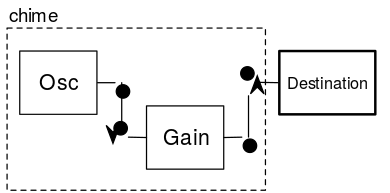
\includegraphics[scale=0.35]{chime.png}
\caption{Estrutura de síntese da API webaudio. \textbf{Fonte}: \cite{srikumar_tamming_2013}.}
\label{fig:shime}
\end{figure}

\subsection{Script Processor Node}

Um sintetizador mais complexo contêm diversos nós concatenados. Este sintetizador complexo pode ser simplificado com um outro nó, chamado \emph{ScriptProcessorNode}. Uma instância deste nó permite o cálculo customizado de cada \emph{sample} em um \emph{buffer}, à semelhança de uma função matemática. 

\subsection{GROOVE}

Este artigo envolve uma pesquisa sobre prática \emph{livecoding} \cite{collins_origins_2014,prospero_social_2015,prospero_social_2015}. 

O resultado deste artigo não é o objetivo da pesquisa, mas relaciona uma proposta histórica de Max Mathews, \cite{mathews_groove_1970}, GROOVE. O estudo deste trabalho de Mathews foi fundamental para o entendimento de um paradigma do \emph{livecoding}: ao digitar comandos em um console de computador, é possível ouvir os os resultados, e modificá-los através de novos comandos, e/ou com controles externos. 

Para que este modelo de paradigma fosse aplicado em um navegador de internet, recorremos à implementação do \emph{ScriptProcessorNode}, da equipe desenvolvedora do programa \emph{Wavepot}\footnote{Disponível em \url{http://www.wavepot.com}.}. 

%A Seção \ref{sec:trabalhos} deste artigo apresenta os frameworks supracitados e uma breve comparação entre eles.
%A Seção \ref{sec:termpot} apresenta a ferramenta proposta.
%A Seção \ref{sec:resultados} traz os resultados desta pesquisa e a Seção \ref{sec:conclusao} apresenta as conclusões do trabalho até o presente momento.

